\documentclass[tikz,border=7pt]{standalone}
\usepackage{amsmath}
\usetikzlibrary{arrows.meta,positioning}

\definecolor{ink}{HTML}{21352F}
\definecolor{teal}{HTML}{087F7B}
\definecolor{rose}{HTML}{B65A62}
\definecolor{gold}{HTML}{C58B2A}
\definecolor{blue}{HTML}{4B77A8}

\begin{document}
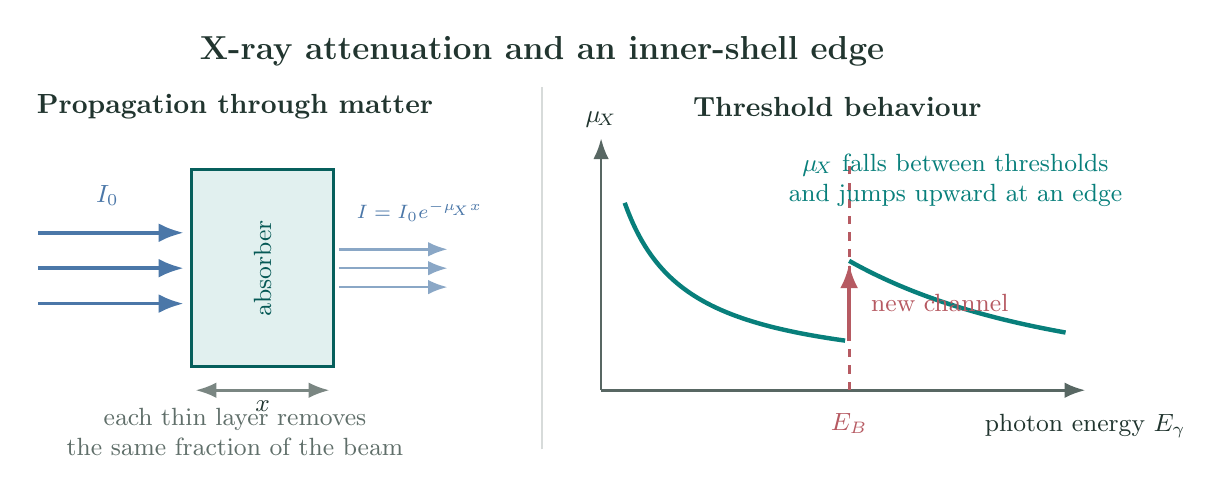
\begin{tikzpicture}[font=\sffamily,>=Latex]
  \node[font=\bfseries\large,text=ink] at (0,2.75)
    {X-ray attenuation and an inner-shell edge};

  % Attenuating slab
  \node[font=\bfseries,text=ink] at (-3.9,2.05)
    {Propagation through matter};
  \foreach \y in {-0.45,0,0.45}{
    \draw[->,line width=1.35pt,draw=blue]
      (-6.4,\y) -- (-4.55,\y);
  }
  \node[text=blue,font=\small] at (-5.52,0.92) {$I_0$};

  \fill[teal!12] (-4.45,-1.25) rectangle (-2.65,1.25);
  \draw[line width=1.2pt,draw=teal!75!black]
    (-4.45,-1.25) rectangle (-2.65,1.25);
  \draw[<->,line width=1pt,draw=ink!60]
    (-4.4,-1.55) -- (-2.7,-1.55)
    node[midway,below,text=ink,font=\small] {$x$};
  \node[rotate=90,text=teal!70!black,font=\small] at (-3.55,0)
    {absorber};

  \foreach \y in {-0.24,0,0.24}{
    \draw[->,line width=0.9pt,draw=blue!65]
      (-2.58,\y) -- (-1.2,\y);
  }
  \node[anchor=west,text=blue,font=\scriptsize] at (-2.48,0.72)
    {$I=I_0e^{-\mu_{\!X}x}$};
  \node[align=center,text=ink!72,font=\small] at (-3.9,-2.08)
    {each thin layer removes\\the same fraction of the beam};

  \draw[ink!18,line width=1pt] (0,-2.3) -- (0,2.3);

  % Absorption coefficient versus photon energy
  \node[font=\bfseries,text=ink] at (3.75,2.05)
    {Threshold behaviour};
  \draw[->,line width=1pt,draw=ink!75]
    (0.75,-1.55) -- (6.9,-1.55)
    node[below=5pt,text=ink,font=\small] {photon energy $E_\gamma$};
  \draw[->,line width=1pt,draw=ink!75]
    (0.75,-1.55) -- (0.75,1.65)
    node[above,text=ink,font=\small] {$\mu_{\!X}$};

  % Between thresholds the photoelectric contribution falls with energy.
  \draw[line width=1.6pt,draw=teal,domain=0.15:2.95,samples=90,smooth,
        variable=\x]
    plot ({0.9+\x},{-1.42+1.8/(\x+0.65)});
  \draw[line width=1.6pt,draw=teal,domain=3.0:5.75,samples=90,smooth,
        variable=\x]
    plot ({0.9+\x},
      {-1.42+1.8/(\x+0.65)+1.02*exp(-0.42*(\x-3.0))});

  \draw[dashed,draw=rose,line width=1pt] (3.9,-1.55) -- (3.9,1.35);
  \draw[->,line width=1.25pt,draw=rose]
    (3.9,-0.92) -- (3.9,0.05)
    node[midway,right=4pt,text=rose,font=\small] {new channel};
  \node[below=5pt,text=rose,font=\small] at (3.9,-1.55) {$E_B$};
  \node[text=teal,font=\small,align=center] at (5.25,1.12)
    {$\mu_{\!X}$ falls between thresholds\\and jumps upward at an edge};
\end{tikzpicture}
\end{document}
